\documentclass[journal,12pt,twocolumn]{IEEEtran}

\usepackage{setspace}
\usepackage{gensymb}
\singlespacing
\usepackage[cmex10]{amsmath}
\usepackage{caption}

\usepackage{amsthm}

\usepackage{mathrsfs}
\usepackage{txfonts}
\usepackage{stfloats}
\usepackage{bm}
\usepackage{cite}
\usepackage{cases}
\usepackage{subfig}

\usepackage{longtable}
\usepackage{multirow}

\usepackage{enumitem}
\usepackage{mathtools}
\usepackage{steinmetz}
\usepackage{tikz}
\usepackage{circuitikz}
\usepackage{verbatim}
\usepackage{tfrupee}
\usepackage[breaklinks=true]{hyperref}
\usepackage{graphicx}
\usepackage{tkz-euclide}

\usetikzlibrary{calc,math}
\usepackage{listings}
    \usepackage{color}                                            %%
    \usepackage{array}                                            %%
    \usepackage{longtable}                                        %%
    \usepackage{calc}                                             %%
    \usepackage{multirow}                                         %%
    \usepackage{hhline}                                           %%
    \usepackage{ifthen}                                           %%
    \usepackage{lscape}     
\usepackage{multicol}
\usepackage{chngcntr}

\DeclareMathOperator*{\Res}{Res}

\renewcommand\thesection{\arabic{section}}
\renewcommand\thesubsection{\thesection.\arabic{subsection}}
\renewcommand\thesubsubsection{\thesubsection.\arabic{subsubsection}}

\renewcommand\thesectiondis{\arabic{section}}
\renewcommand\thesubsectiondis{\thesectiondis.\arabic{subsection}}
\renewcommand\thesubsubsectiondis{\thesubsectiondis.\arabic{subsubsection}}


\hyphenation{op-tical net-works semi-conduc-tor}
\def\inputGnumericTable{}                                 %%

\lstset{
%language=C,
frame=single, 
breaklines=true,
columns=fullflexible
}
\begin{document}


\newtheorem{theorem}{Theorem}[section]
\newtheorem{problem}{Problem}
\newtheorem{proposition}{Proposition}[section]
\newtheorem{lemma}{Lemma}[section]
\newtheorem{corollary}[theorem]{Corollary}
\newtheorem{example}{Example}[section]
\newtheorem{definition}[problem]{Definition}

\newcommand{\BEQA}{\begin{eqnarray}}
\newcommand{\EEQA}{\end{eqnarray}}
\newcommand{\define}{\stackrel{\triangle}{=}}
\bibliographystyle{IEEEtran}
\raggedbottom
\setlength{\parindent}{0pt}
\providecommand{\mbf}{\mathbf}
\providecommand{\pr}[1]{\ensuremath{\Pr\left(#1\right)}}
\providecommand{\qfunc}[1]{\ensuremath{Q\left(#1\right)}}
\providecommand{\sbrak}[1]{\ensuremath{{}\left[#1\right]}}
\providecommand{\lsbrak}[1]{\ensuremath{{}\left[#1\right.}}
\providecommand{\rsbrak}[1]{\ensuremath{{}\left.#1\right]}}
\providecommand{\brak}[1]{\ensuremath{\left(#1\right)}}
\providecommand{\lbrak}[1]{\ensuremath{\left(#1\right.}}
\providecommand{\rbrak}[1]{\ensuremath{\left.#1\right)}}
\providecommand{\cbrak}[1]{\ensuremath{\left\{#1\right\}}}
\providecommand{\lcbrak}[1]{\ensuremath{\left\{#1\right.}}
\providecommand{\rcbrak}[1]{\ensuremath{\left.#1\right\}}}
\theoremstyle{remark}
\newtheorem{rem}{Remark}
\newcommand{\sgn}{\mathop{\mathrm{sgn}}}
\providecommand{\abs}[1]{\left\vert#1\right\vert}
\providecommand{\res}[1]{\Res\displaylimits_{#1}} 
\providecommand{\norm}[1]{\left\lVert#1\right\rVert}
%\providecommand{\norm}[1]{\lVert#1\rVert}
\providecommand{\mtx}[1]{\mathbf{#1}}
\providecommand{\mean}[1]{E\left[ #1 \right]}
\providecommand{\fourier}{\overset{\mathcal{F}}{ \rightleftharpoons}}
%\providecommand{\hilbert}{\overset{\mathcal{H}}{ \rightleftharpoons}}
\providecommand{\system}{\overset{\mathcal{H}}{ \longleftrightarrow}}
 %\newcommand{\solution}[2]{\textbf{Solution:}{#1}}
\newcommand{\solution}{\noindent \textbf{Solution: }}
\newcommand{\cosec}{\,\text{cosec}\,}
\providecommand{\dec}[2]{\ensuremath{\overset{#1}{\underset{#2}{\gtrless}}}}
\newcommand{\myvec}[1]{\ensuremath{\begin{pmatrix}#1\end{pmatrix}}}
\newcommand{\mydet}[1]{\ensuremath{\begin{vmatrix}#1\end{vmatrix}}}
\numberwithin{equation}{subsection}
\makeatletter
\@addtoreset{figure}{problem}
\makeatother
\let\StandardTheFigure\thefigure
\let\vec\mathbf
\renewcommand{\thefigure}{\theproblem}
\def\putbox#1#2#3{\makebox[0in][l]{\makeb
ox[#1][l]{}\raisebox{\baselineskip}[0in][0in]{\raisebox{#2}[0in][0in]{#3}}}}
     \def\rightbox#1{\makebox[0in][r]{#1}}
     \def\centbox#1{\makebox[0in]{#1}}
     \def\topbox#1{\raisebox{-\baselineskip}[0in][0in]{#1}}
     \def\midbox#1{\raisebox{-0.5\baselineskip}[0in][0in]{#1}}
\vspace{3cm}
\title{Assignment 2}
\author{Tarandeep Singh}
\maketitle
\newpage
\bigskip
\renewcommand{\thefigure}{\theenumi}
\renewcommand{\thetable}{\theenumi}
Github Link
\begin{lstlisting}
https://github.com/Tarandeep97/AI5030
\end{lstlisting}
\section{Problem}
(52) Suppose X$\sim$ Cauchy(0,1). Then the distribution of
$\frac{1-X}{1+X}$ is?
\section{Solution}
A continuous random variable X follows \textbf{Cauchy distribution} with parameters $\mu$ and $\lambda$ if its pdf is given by
\\
    \begin{equation*} f(x) =\left\{ \begin{array}{ll} \frac{\lambda}{\pi}\cdot \frac{1}{\lambda^2+(x-\mu)^2}, & \hbox{$-\infty < x< \infty$;} \\ & \hbox{$-\infty < \mu< \infty$, $\lambda>0$;} \\ 0, & \hbox{Otherwise.} \end{array} \right. \end{equation*}
    
\\
The parameter $\mu$ and $\lambda$ are location and scale parameters respectively. 
\\
When $\mu$=0 and $\lambda$=1, then the distribution is called \textbf{Standard Cauchy Distribution}. The pdf of standard Cauchy distribution is
\\
\begin{equation*} f(x) =\left\{ \begin{array}{ll} \frac{1}{\pi}\cdot \frac{1}{1+x^2}, & \hbox{$-\infty < x< \infty$;} \\ 0, & \hbox{Otherwise.} \end{array} \right. \end{equation*}

Let,
\begin{align}
    Y = \frac{1-X}{1+X}
\end{align}
Then, cdf of Y is
\begin{align}
    F_{Y}(y) = P(Y \leq y)
\end{align}
\begin{align}
    = P\left(\frac{1-X}{1+X} \leq y\right)
\end{align}
\begin{align}
    = P\left((1-X) \leq y.(1+X)\right)
\end{align}
\begin{align}
    = P\left((1-X) \leq (y+y.X)\right)
\end{align}
\begin{align}
    = P\left((1-y) \leq (X+y.X)\right)
\end{align}
\begin{figure}[ht]
\centering
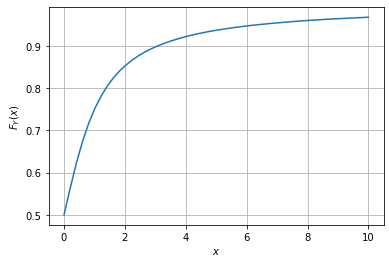
\includegraphics[width=\columnwidth]{cdf.png}
\caption*{Fig 1. CDF of Y}
\label{fig:fig1}
\end{figure}
\begin{figure}[ht]
\centering
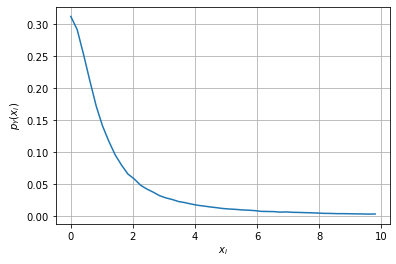
\includegraphics[width=\columnwidth]{pdf.png}
\caption*{Fig 2. PDF of Y}
\label{fig:fig2}
\end{figure}
\begin{align}
    = P\left(\frac{1-y}{1+y} \leq X \right)
\end{align}
\begin{align}
    = 1 - P\left(X < \frac{1-y}{1+y}\right)
\end{align}
\begin{align}
    = 1 -  \int_{-\infty}^{\frac{1-y}{1+y}} f(x) \,dx
\end{align}
\begin{align}
    = 1 -  \int_{-\infty}^{\frac{1-y}{1+y}} \frac{1}{\pi}\cdot \frac{1}{1+x^2} \,dx
\end{align}
\begin{align}
    = 1 -  \frac{1}{\pi}\cdot \left[tan^{-1}x\right]_{-\infty}^{\frac{1-y}{1+y}}
\end{align}
\begin{align}
    = 1 -  \frac{1}{\pi}\cdot \left[\left[tan^{-1}x\right]_{-\infty}^{0}+\left[tan^{-1}x\right]_{0}^{\frac{1-y}{1+y}}\right]
\end{align}
\begin{align}
    = 1 -  \frac{1}{\pi}\cdot \left[-\frac{\pi}{2}+\left[tan^{-1}x\right]_{0}^{\frac{1-y}{1+y}}\right]
\end{align}
\begin{align}
    F_{Y}(y) = 1 -  \frac{1}{\pi}\cdot \left[-\frac{\pi}{2}+tan^{-1}\left({\frac{1-y}{1+y}}\right)\right]
\end{align} \\


The pdf of Y is
\begin{align}
    f_{Y}(y) = \frac{d F_{Y}(y)}{dy} = -\frac{1}{\pi}\cdot\frac{d\left(tan^{-1}\left({\frac{1-y}{1+y}}\right)\right)}{dy}
\end{align}
\begin{align}
    = -\frac{1}{\pi}\cdot\frac{1}{1+\left(\frac{1-y}{1+y}\right)^{2}}\cdot\frac{d\left({\frac{1-y}{1+y}}\right)}{dy}
\end{align}
\begin{align}
    = -\frac{1}{\pi}\cdot\frac{1}{1+\left(\frac{1-y}{1+y}\right)^{2}}\cdot\left( -\frac{2}{\left(y + 1\right)^{2}}\right)
\end{align}
\begin{align}
    = \frac{1}{\pi}\cdot \frac{1}{1+y^2}
\end{align}
Hence,  Y $\sim$ Cauchy(0,1).\\


\end{document}
